\documentclass[xcolor=table]{beamer}

%\usepackage[table]{xcolor}
\usepackage{amssymb} 
\usepackage{amsmath}
\usepackage{graphicx} 
\usepackage{hyperref}
%\usepackage{booktabs}
\usepackage{float}

%\usepackage{caption}
%\usepackage{beamerthemesplit} %questo fa uscire il summary al top che si mangia mezza slide... \useinnertheme{default} \usetheme{Marburg} %Warsaw
%Marburg %Montpellier

%%%%%%%%% NEW COMMAND MACRO %%%%%%%%%%%%%%%%%%%%%%%%%%%%%%

\newcommand{\notorth}{\ensuremath{\perp\!\!\!\!\!\!\diagup\!\!\!\!\!\!\perp}}
\newcommand{\orth}{\ensuremath{\perp\!\!\!\perp}}

%%%%%%%%%%%%%%%%%%%%%%%%%%%%%%%%%%%%%%%%%%%%%%%%%%%%%%%%%%

\setbeamerfont{table}{size=\footnotesize} 
\setbeamerfont{smalltable}{size=\scriptsize} 
\setbeamerfont{microtable}{size=\tiny}
\setbeamertemplate{navigation symbols}{}  %%Get rid of the navigation symbols at the bottom
\setbeamertemplate{footline}[text line]{\parbox{\linewidth}{\hfill  \insertpagenumber / \insertpresentationendpage}} %\insertshortauthor \hspace{2ex} \insertshorttitle
\usepackage{booktabs}
\usepackage[flushleft]{threeparttable}

% Alternatively, you can try Copenhagen; its borders are slightly less dark, but its the same style (rounded edged rectangle on the first %slide)
%\usetheme{Copenhagen}

%Next two lines are stuff that was already here. 
\setbeamertemplate{mini frames}[default] 
\setbeamertemplate{mini frame in other subsection}[default][20]

%Here is alternative table of contents pointers% 
\setbeamertemplate{sections/subsections in toc}[square] 
%\setbeamertemplate{sections/subsections in toc}[circle] 
%\setbeamertemplate{sections/subsections in toc}[ball] 
%\setbeamertemplate{sections/subsections in toc}[ball unnumbered]
%\setbeamertemplate{sections/subsections in toc}[default]

%The next line is the background. Right now we have it set to a vertical shading, with top white bottom 20% blue. 
%You can alter this however you want. We were using red!20 before. You can use standard names for colors, or if I understand correctly 
%you can also use RGB (red green blue) code, for example 30,30,30) 
%\setbeamertemplate{background canvas}[vertical shading][top=white,bottom=blue!10]

%Alternatively, you can make the background just a solid color. 
%\setbeamercolor{background canvas}{bg=red!5}

%Below is the amount of opaqueness in terms of percent.  You can remove this line or set to 0 and it will make future lines unable to be seen.
\setbeamercovered{transparent=15}

%stuff from before \setbeamersize{<text margin left=0.1 in>, <text margin right=.1 in>, <sidebar width left=0 in>, <sidebar width right=0 in>} %
%%%%%%%%%%%%%%%%%%%%%%%%%%%%%%%%%%%%%%%%%%%%%%%%%%%%%%%%%%%%%%%%%%%%%%%%%%%%%%%

\graphicspath{{../../presentation/include/}{./}}
\makeatletter
\def\input@path{{../../presentation/include/}{./}}
\makeatother

\title[Reggio Children Approach]{Reggio Children: Survey Design and Data Collection} 
\bigskip
\subtitle{The Reggio Children Approach}
%\usebeamerfont{smalltable}
\author[ReggioTeam]{The Reggio Team}
\date{\today}

\begin{document}

%------------------------------------------------------------------------%
\frame{\titlepage}

\AtBeginSection[]{
  \frame<beamer>{ 
    \frametitle{Outline}   
    \tableofcontents[currentsection,currentsubsection] 
                }
}

\section{Introduction}\label{sec:Intro}
%%------------------------------------------------------------------------------------------------------- 
\begin{frame}
\frametitle{Research Question} 
\begin{itemize}
	\item Importance of early years established by interdisciplinary literature
	\item Convincing evidence from small-scale RCT
	\vspace{2ex}
	%\pause
	\item[Q:] Can these effects be sustained in high-quality child care brought up to scale?
\end{itemize}
\end{frame}
%%------------------------------------------------------------------------------------------------------- 
\begin{frame}
\frametitle{The Reggio Children Approach to Early Childhood Education} 
\begin{itemize}
\item Natural experiment started 50 years ago in Reggio Emilia
\item Comprehensive program, age 0-6 
\item High-quality but scalable in size and sustainable
\item Span across social and economic classes
\item Both natives and immigrants

\vspace{4ex}

\end{itemize}
\end{frame} 
%%------------------------------------------------------------------------------------------------------- 
\begin{frame}
\frametitle{Challenges} 
\begin{itemize}
	\item Non-randomized $\Rightarrow$ construct control group
	\item Long-lasting and evolving program $\Rightarrow$ varying over time
	\item Potential spillovers
\end{itemize}
\end{frame}

\subsection{Early Childhood Education in Italy}\label{sec:ECE_IT}
%%----------------------------------------------------------------------------------------------- 
\begin{frame}
\frametitle{Early Childhood Education in Italy}\label{frame:ECE_IT}
%\usebeamerfont{table}
\begin{itemize}
	\item 4 institutional types: \hyperlink{fig:PrivateAsiloIT}{\beamergotobutton{asilo}}
	\begin{enumerate}
		\item Municipal
		\item State
		\item Religious
		\item Private
	\end{enumerate}
	\vspace{1ex}
	\item 2 age groups: \hyperlink{fig:AttendaceAsiloIT}{\beamergotobutton{asilo}}
	\begin{enumerate}
		\item Age 0-2: 13\% attendance rate (\textit{asilo nido})
		\item Age 3-5: 94\% attendance rate (\textit{scuola materna})
	\end{enumerate}
	
	\vspace{3ex}
	
	\item[] Reggio Children Approach: \textbf{municipal} infant-toddler centers and preschools \textbf{(age 0-5)} in \textbf{Reggio Emilia}
\end{itemize} 
\end{frame} 
%%-----------------------------------------------------------------------------------------------
\begin{frame}
\frametitle{Treatment and Control Groups}
%\documentclass{article}
%
%\usepackage{booktabs}
%\usepackage{float}
%\usepackage[table]{xcolor}
%
%\begin{document}

\begin{table}
\begin{center}
\begin{tabular}{ccccccc}
\toprule
& \multicolumn{3}{c}{Infant-Toddler (0-3)} & \multicolumn{3}{c}{Preschool (3-5)} \\
& Reggio & Parma & Padova & Reggio & Parma & Padova \\
\midrule
Municipal 	& \textbf{T} & \cellcolor{black!20}C & \cellcolor{black!20}C & \textbf{T} & \cellcolor{black!20}C & \cellcolor{black!20}C \\
State 	& 	&  & & \cellcolor{black!20}C & \cellcolor{black!20}C & \cellcolor{black!20}C \\
Religious 	& \cellcolor{black!20}C & \cellcolor{black!20}C & \cellcolor{black!20}C & \cellcolor{black!20}C & \cellcolor{black!20}C & \cellcolor{black!20}C \\
Private 	& \cellcolor{black!20}C & \cellcolor{black!20}C & \cellcolor{black!20}C & \cellcolor{black!20}C & \cellcolor{black!20}C & \cellcolor{black!20}C \\
None 	& \cellcolor{black!20}C & \cellcolor{black!20}C & \cellcolor{black!20}C & \cellcolor{black!20}C & \cellcolor{black!20}C & \cellcolor{black!20}C \\
\bottomrule
\end{tabular}
\caption{In this table, \textbf{T} denotes the treatment group and \textbf{C} denotes the control group. The treatment group is the municipal infant-toddler care and preschool care given in Reggio. This is what is commonly referred to as the ``Reggio" intervention. The municipal school was only widely available for Cohorts I-IV (approximately ages 6 to mid-40s at the time of interview). In addition to the municipal school there is also other types of infant-toddler care and preschools (state, religious, private, none). An exception is that there is no state infant-toddler care.}
\end{center}
\end{table}

%\end{document}

\end{frame}
%%-----------------------------------------------------------------------------------------------
\section{The Reggio Children Approach}\label{sec:RCH}
%%----------------------------------------------------------------------------------------------- 
\begin{frame}
\frametitle{The Reggio Children Approach - Philosophy}\label{frame:philosphy}
%\usebeamerfont{table}
\begin{itemize}
	\item Reggio Children Approach: educational philosophy started by \textbf{Loris Malaguzzi} after World War II.
	\item First preschool 1963; first infant-toddler center 1972
	\item Famous and replicated all over the world \hyperlink{fig:World}{\beamergotobutton{map}}
	\item 26 Infant-toddler centers and 30 preschools
	\vspace{2ex}
	\item Three main pillars:
		\begin{itemize}
%		\usebeamerfont{smalltable}
	\item The organization of the class and the training and collegial work for all educational figures.
	\item The central role of children and the important role of families.
	\item A strong creative, aesthetic and environmental dimension.
		\end{itemize} 
\end{itemize} 
\end{frame} 
%%-----------------------------------------------------------------------------------------------
\begin{frame}
\frametitle{Reggio Children Infant-Toddler Centers (0-3)}
\begin{center}
\begin{figure}
\includegraphics[width=1.0\textheight]{Num_Nidi.pdf}
\caption{No. of children (0-3) in municipal infant-toddler centers.}
\end{figure}
\end{center}
\end{frame}
%%-----------------------------------------------------------------------------------------------
\begin{frame}
\frametitle{Reggio Children Infant-Toddler Centers (0-3)}
\begin{center}
\begin{figure}
\includegraphics[width=1.0\textheight]{Prop_Nidi.pdf}
\caption{\% of children (0-3) in municipal infant-toddler centers.}
\end{figure}
\end{center}
\end{frame} 
%%-----------------------------------------------------------------------------------------------
\begin{frame}
\frametitle{Reggio Children Preschools (3-5)}
\begin{center}
\begin{figure}
\includegraphics[width=1.0\textheight]{Num_Scuole.pdf}
\caption{No. of children (3-5) in municipal preschools.}
\end{figure}
\end{center}
\end{frame} 
%%-----------------------------------------------------------------------------------------------
\begin{frame}
\frametitle{Reggio Children Preschools (3-5)}
\begin{center}
\begin{figure}
\includegraphics[width=1.0\textheight]{Prop_Scuole.pdf}
\caption{\% of children (3-5) in municipal preschools.}
\end{figure}
\end{center}
\end{frame} 

\section{Administrative Data Collected}
%\subsection{Administrative Data}
%%-----------------------------------------------------------------------------------------------
\begin{frame}
\frametitle{Administrative Data}
\usebeamerfont{table}
For \textbf{all} the children who have applied to the Reggio municipal preschools from 2003-2010 (n=10,841) we have unique information from:
\begin{itemize}
\item\underline{application forms}: place of residence, family composition, early child care;
\item\underline{interview with the parents}: child's verbal language, play/free-time activities, motor abilities, eating and sleeping habits, and general health status;
\item\underline{interview among teachers}: start and end of preschool
\item\underline{teachers' reports}: child cognitive and socioemotional development.
\item\underline{attendance list}: names of children who attended the centers
\end{itemize}

\vspace{2ex}
Who can apply?
\begin{itemize}
	\item resident in Reggio Emilia
	\item age 3-4-5
	\item age 2 if born after 30 April and no waiting list
\end{itemize}

%\bigskip
%
%$\Longrightarrow$ \textit{\underline{Revised evaluation design}} -- sample of children 3-5 who attended the Reggio Children preschools:
%\begin{itemize}
%\usebeamerfont{table}
%\item\textbf{treatment group}: children who have previously attended a municipal infant-toddler center;
%\item\textbf{control group}: children who had alternative non-school based child care.
%\end{itemize}
\end{frame}
%---------------------------------------------------------------------------------------------------------------------------------
\begin{frame}
%% This table can be obtained using the dataset: klmReggio/ADMINISTRATIVE DATA COLLECTION/DATI/ReggioAdminData.dta
%% tab anno_scolastico migr_b, row

\begin{table}[ht!]
\caption{\textbf{\small Numbers of Applications to Municipal Preschools}}
\label{tab:NumApps}
%\vspace{-5mm}
\begin{center}
\begin{tabular}{ccc}
\hline\hline
\textbf{School Year} & \textbf{Applications (\#)} & \textbf{Immigrants (\%)} \\
\hline
2003-2004 & 1,228 & 13.4 \\[0.2em]
2004-2005 & 1,312 & 14.3 \\[0.2em]
2005-2006 & 1,442 & 19.4 \\[0.2em]
2006-2007 & 1,409 & 18.7 \\[0.2em]
2007-2008 & 1,349 & 20.8 \\[0.2em]
2008-2009 & 1,418 & 22.1 \\[0.2em]
2009-2010 & 1,352 & 23.2 \\[0.2em]
2010-2011 & 1,331 & 28.1 \\[0.2em]
\hline
\end{tabular}
\end{center}
\begin{flushleft}
\tiny{{\bfseries Notes:} Source: authors' calculations from the administrative data on the universe of applications to the municipal preschools of Reggio Emilia. The first column reports the school year the application refers to; the second column reports the number of applications to the municipal preschools received in that school year; the third column reports the percentage of applications made for immigrant children.}
\end{flushleft}
\end{table}

\end{frame}
%---------------------------------------------------------------------------------------------------------------------------------
\begin{frame}
%% This table can be obtained using the dataset: klmReggio/ADMINISTRATIVE DATA COLLECTION/DATI/ReggioAdminData.dta
%% tab anno_scolastico bam_scol, row

\begin{table}[ht!]
\caption{\textbf{\small Outcome of Applications to Municipal Preschools}}
\label{tab:OutcApps}
%\vspace{-5mm}
\begin{center}
\begin{tabular}{c c c c c }
\hline\hline
\textbf{School Year} & \textbf{Attended} & \textbf{Withdrew} & \textbf{Waitlist} & \textbf{Refused} \\
\hline
        2003-2004  &   48.3  &    42.8  &    2.9  &    6.0   \\[0.2em]
        2004-2005  &   48.3  &    36.9  &    6.2  &    8.6   \\[0.2em]
        2005-2006  &   60.1  &    20.0  &    8.1  &   11.9   \\[0.2em]
        2006-2007  &   52.8  &    24.8  &   13.4  &    8.9   \\[0.2em]
        2007-2008  &   48.5  &    20.9  &   23.4  &    7.1   \\[0.2em]
        2008-2009  &   53.4  &     1.3  &   35.6  &    9.8   \\[0.2em]
        2009-2010  &   52.2  &     2.1  &   36.2  &    9.6   \\[0.2em]
        2010-2011  &   53.5  &     1.9  &   37.1  &    7.5   \\[0.2em]
\hline
\textit{Total} &   \textit{52.2 \%} &   \textit{18.4 \%} &   \textit{20.6 \%} &    \textit{8.7 \%}  \\[0.2em]
\hline
\end{tabular}
\end{center}
\begin{flushleft}
\tiny{{\bfseries Notes:} Source: authors' calculations from the administrative data on the universe of applications to the municipal preschools of Reggio Emilia. The cells display the percentages of applications for that particular school year which had that particular outcome: the child attended the assigned preschool (column 1); the child withdrew from the municipal preschool system (either because she went to another preschool or stayed home) after being accepted but before being assigned a specific preschool (column 2); the child was on waiting list (column three); the child dropped out from the municipal school system after a specific preschool was assigned (column 4).}
\end{flushleft}
\end{table}

\end{frame}
%---------------------------------------------------------------------------------------------------------------------------------
\begin{frame}
%% This table can be obtained using the dataset: klmReggio/ADMINISTRATIVE DATA COLLECTION/DATI/ReggioAdminData.dta
%% gen year_begin = anno-anno_nas
%% tab anno_scolastico year_begin , row

\begin{table}[ht!]
\caption{\textbf{\small Age of Applicants to Municipal Preschools, by School Year}}
\label{tab:AgeApps}
%\vspace{-5mm}
\begin{center}
\begin{tabular}{ c c c c }
\hline\hline
\textbf{School Year} & \textbf{Age 3 (\%)} & \textbf{Age 4 (\%)} & \textbf{Age 5 (\%)} \\
\hline
	2003-2004  &  81.9  &    11.8  &    6.0   \\[0.2em]
	2004-2005  &  77.4  &    14.6  &    7.8   \\[0.2em]
	2005-2006  &  73.3  &    12.7  &   11.5   \\[0.2em]
	2006-2007  &  74.4  &    14.9  &    8.7   \\[0.2em]
	2007-2008  &  79.6  &    11.2  &    8.2   \\[0.2em]
	2008-2009  &  76.6  &    14.3  &    9.1   \\[0.2em]
	2009-2010  &  79.2  &    11.0  &    7.9   \\[0.2em]
	2010-2011  &  77.5  &    13.0  &    7.1   \\[0.2em]
\hline
	\textit{Total}  &  \textit{77.4 \% } & \textit{12.9 \% } & \textit{8.3 \%}   \\[0.2em]
\hline
\end{tabular}
\end{center}
\begin{flushleft}
\tiny{{\bfseries Notes:} Source: authors' calculations from the administrative data on the universe of applications to the municipal preschools of Reggio Emilia. The cells display the percentages of applicants who were 3, 4 and 5 years-old when applying to each school year. The age is calculated based on the year of birth of the child, so that for example children born any time in 2005 are considered 3-year-old if applying to the 2008-2009 School Year.}
\end{flushleft}
\end{table}

\end{frame}
%---------------------------------------------------------------------------------------------------------------------------------
\begin{frame}
% use KlmReggio\ADMINISTRATIVE DATA COLLECTION\DATI\ReggioAdminData.dta
% from summaryStat.do
%   estpost tabstat $var_compare, by (migr_b)  statistics(mean sd) columns(statistics)
%   esttab using AdminSum_migr.tex, $options coef($AdminLabel)
%
\begin{table}[!ht]
\caption{\textbf{Administrative Data Summary Statistics, Italian and Immigrant Children}}
\label{tab:AdminSum}
\begin{center}
\scriptsize

\begin{tabular}{l*{3}{c}} \hline\hline
             &     \textbf{Italian}  &     \textbf{Migrant}  &       \textbf{Total}\\
\hline
Female       &       48.6\%  &       44.8\%  &       47.8\%\\
             &     (50.0)  &     (49.7)  &     (50.0)\\
%Migrant Father  &       0.1  &       0.8  &       0.2\\
%              &     (0.2)  &     (0.4)  &     (0.4)\\
%Migrant Mother  &       0.1  &       0.9  &       0.3\\
%              &     (0.3)  &     (0.4)  &     (0.4)\\
Child born in Reggio  &       67.8\%  &       67.8\%  &       67.8\% \\
              &     (46.7)  &     (46.7)  &     (46.7) \\
Lives in Reggio  &       98.4\%  &       99.6\%  &       98.6\%\\
              &     (12.6)  &     (6.1)  &     (11.6)\\
%Father born in Reggio  &       0.3  &       0.1  &       0.3\\
%              &     (0.5)  &     (0.3)  &     (0.5)\\
%Mother born in Reggio  &       0.4  &       0.0  &       0.3\\
%              &     (0.5)  &     (0.2)  &     (0.5)\\
Intact Family  &       94.8\%  &       86.6\%  &       93.6\%\\
              &     (22.2)  &     (34.2)  &     (24.5)\\
Father low education  &       39.3\%  &       52.1\%  &       41.5\%\\
              &     (48.8)  &     (50.0)  &     (49.3)\\
%Father high school grad  &       0.4  &       0.4  &       0.4\\
%              &     (0.5)  &     (0.5)  &     (0.5)\\
Father college graduate  &       17.1\%  &      8.8\% &       15.7\%\\
             &     (37.7) &     (28.3) &     (36.4)\\
Mother low education &       28.5\% &       55.7\% &       33.3\%\\
             &     (45.2) &     (49.7) &     (47.1)\\
%Mother high school grad &       0.5 &       0.3 &       0.5\\
%             &     (0.5) &     (0.5) &     (0.5)\\
Mother college graduate &       20.8\% &       9.6\% &       18.9\%\\
             &     (40.6) &     (29.4) &     (39.1)\\
%Asked for priority &       0.5 &       0.5 &       0.5\\
%             &     (0.5) &     (0.5) &     (0.5)\\
%Asked for municipal preschool &       0.9 &       0.8 &       0.9\\
%             &     (0.3) &     (0.4) &     (0.3)\\
%Adopted      &       0.0 &       0.0 &       0.0\\
%             &     (0.1) &     (0.1) &     (0.1)\\
% Number of siblings &       1.10 &       1.28 &       1.14 \\
             % &     (0.71) &     (0.81) &     (0.73)\\
% Father works &       94.6\% &       90.2\% &       93.8\%\\
             % &     (22.5) &     (29.8) &     (24.2)\\
%Father working hours &      41.2 &      39.9 &      40.9\\
%             &     (7.2) &     (3.9) &     (6.7)\\
% Mother works &       72.6\% &       42.2\% &       66.7\%\\
             % &     (44.6) &     (49.4) &     (47.1)\\
%Mother working hours &      33.8 &      33.4 &      33.7\\
%             &     (8.7) &    (10.2) &     (8.9)\\
%ISEE         &     1.3e+04 &    4924.6 &     1.1e+04\\
%             &  (7319.4) &  (4307.7) &  (7532.8)\\
% Primary Score &      25.0 &      20.5 &      24.1\\
             % &    (13.9) &    (15.1) &    (14.2)\\
% Secondary Score &      29.4 &      30.7 &      29.6\\
             % &    (14.9) &    (18.8) &    (15.7)\\
Child accepted &       82.8\% &       65.7\% &       79.4\%\\
             &     (37.7) &     (47.5) &     (40.5)\\
\hline
\(N\)        &       8,525 &      2,145  &      10,670 \\
\hline
\end{tabular}
\end{center}
\begin{flushleft}
\tiny{
{\bfseries Notes:} Source: authors' calculations from the administrative data on the universe of applications to the municipal preschools of Reggio Emilia. Standard deviations in parenthesis. ``Low education'' includes no schooling, elementary schooling, and middle-high schooling.}
\end{flushleft}
\end{table}


\end{frame}
%: Reggio Score
%%-----------------------------------------------------------------------------------------------
\begin{frame}
\frametitle{Reggio Children Applications}\label{frame:ReggioScore}

\begin{itemize}
	\item Applications submitted on January
	\item Two scores to determine waiting list priority
	%\pause
	\vspace{1ex}
	\item \textbf{Priority}: disability; single teen-age parent; other distress in parenting (illness, death..)
	\item \textbf{Primary Score}: 0-100
	\begin{itemize}
		\item Single parent (14-18 points)
		\item Parental working hours (part time 7 pts, full time 14)
		\item Siblings (older 1 pt, younger at home 5 pts)
		\item Previous child-care attendance (1 to 2 pts)
		\item Family need: illness, work travel, migrants, adpotion (up to 14pt)
		\item Socio-economic distress: unemployed (up to 8pts)
	\end{itemize}
\end{itemize}
\end{frame}
%%-----------------------------------------------------------------------------------------------
\begin{frame}
\frametitle{Reggio Children Primary Score}
\begin{center}
\begin{figure}
\includegraphics[width=1.1\textheight]{PrimaryScore_admin.pdf}
%\caption{Primary Score from administrative data}
\end{figure}
\end{center}
\end{frame}
%%-----------------------------------------------------------------------------------------------
\begin{frame}
\frametitle{Reggio Children Seconday Score}\label{frame:ReggioScore2}
Secondary score based on grand-parents availability
\begin{itemize}
	\item Secondary score: 0-50
	\begin{itemize}
		\item Unavailable: illness, living far, old, working (upt to 12 pts)
		\item Partially available (up to 6pts)
		\item Available (0 pts if living together, 5 if living nearby).
	\end{itemize}
\end{itemize}
\end{frame}
%%-----------------------------------------------------------------------------------------------
\begin{frame}
\frametitle{Reggio Children Secondary Score}
\begin{center}
\begin{figure}
\includegraphics[width=1.1\textheight]{SecondaryScore_admin.pdf}
%\caption{Secondary Score from administrative data}
\end{figure}
\end{center}
\end{frame}

\section{Field Data Collection}
%%-----------------------------------------------------------------------------------------------
\begin{frame}
\frametitle{Sampling Design}
\usebeamerfont{table}
\begin{itemize}
\item\textbf{Stratified sampling design} - strata are defined by cohort, chosen to represent key periods/transitions in the lifecycle:
\begin{itemize}
\usebeamerfont{smalltable}
\item Born 2006 (children entering elementary school);
\item Born 1994 (adolescents reaching maturity);
\item Born 1980-81 (adults at first life milestone);
\item Born 1969-70 (adults at second life milestone; first to have access to infant-todder centers);
\item Born 1954-1959 (adults born before the Reggio Children Approach was implemented).
\end{itemize}
\item Sampling frame taken from population registries (anagrafi)
\item Within each stratum, randomly sample households resident in the city since birth.
\item Screen households to oversample treatment group.
\item A minimum sample size of 150 treated and 150 controls for each stratum has been reached.
\item Professional data collection agency.
\end{itemize}
\end{frame} 
%%-----------------------------------------------------------------------------------------------
\begin{frame}
\frametitle{The Reggio Children Approach - Evaluation} 
\usebeamerfont{table} 
\begin{itemize}

\item\textbf{Treatment group}: attended Reggio Children Schools
\smallskip
\item\textbf{Control groups}: attended other schools or stayed at home
\begin{enumerate}
\usebeamerfont{table}
\item in Reggio Emilia
\item in Parma (Emilia Romagna) 
\item in Padova (Veneto)
\item Across different cohorts
\end{enumerate}
\vspace{3ex}
\item Control cities: comparable to Reggio Emilia in terms of demographics, unemployment and immigration structure
\item Parma: similar culture and history; Padova: different influences
\end{itemize}
\end{frame} 
%%-----------------------------------------------------------------------------------------------
\begin{frame}
\frametitle{Reggio Emilia, Parma, Padova} 
\begin{center}
\begin{figure}
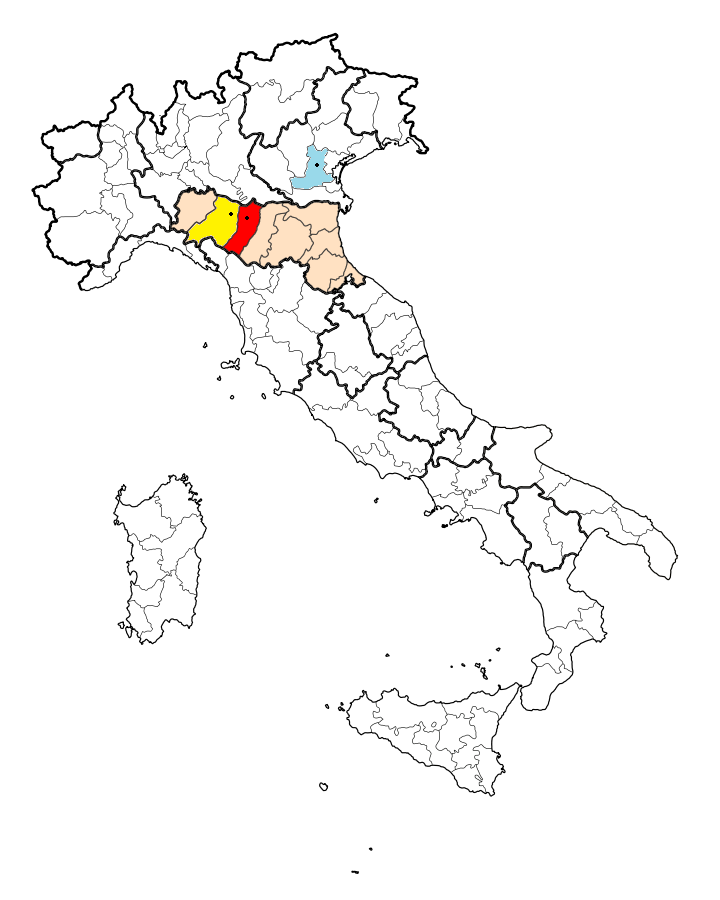
\includegraphics[height=1.0\textheight]{3-cities-map.png}
%\caption{{Location of the city of Parma, Reggio Emilia, and Padova, Italy.}}
\end{figure}
\end{center}
\end{frame}
%---------------------------------------------------------------------------------------------------------------------------------
\begin{frame}
\begin{table}[ht!]
\caption{\textbf{\small Total Reference Sample}}
\label{tab:TotRefSample}
%%\vspace{-5mm}
\begin{center}
\scriptsize
\begin{tabular}{ l c c c c }
\hline\hline
\textbf{Cohort} & \textbf{Reggio} & \textbf{Parma} & \textbf{Padova} & \textbf{Total}\\
\hline
Italian Children born in 2006 (Cohort V)   & 1,096 & 1,054 & 1,224 & 3,374\\[0.2em]
Immigrant Children born in 2006 (Cohort V) &   296 &   224 &   264 &   784\\[0.2em]
Adolescents born in 1994 (Cohort IV)       &   865 &   806 & 1,113 & 2,784\\[0.2em]
Adults born in 1980-81 (Cohort III)        & 1,205 & 1,355 & 1,630 & 4,190\\[0.2em]
Adults born in 1969-70 (Cohort II)         & 1,655 & 2,057 & 2,200 & 5,912\\[0.2em]
Adults born in 1954-59 (Cohort I)          & 3,646 & 3,999 & 5,587 & 13,232\\[0.2em]
\hline
Total                                      & 8,763 & 9,495 & 12,018 & 30,276\\
\hline
\end{tabular}
\end{center}
\begin{flushleft}
\tiny{{\bfseries Notes:} Total number of names provided by the population registries who satisfied the selection criteria (born in the city of residence and of Italian citizenship -- except for Immigrant Children born in 2006), broken down by City and Cohort. Source: authors calculations on data provided by the population registries.}
\end{flushleft}
\end{table} 
\end{frame}
%---------------------------------------------------------------------------------------------------------------------------------
\begin{frame}
\begin{table}[ht!]
\caption{\textbf{Percentage of people living in the same city since birth, by cohort}}
\label{tab:SameCity}
\vspace{-5mm}
\begin{center}
\begin{tabular}{ l c c c c }
\hline\hline
\textbf{Cohort} & \textbf{Reggio (\%)} & \textbf{Parma (\%)} & \textbf{Padova (\%)} & \textbf{Total (\%)}\\
\hline
Italian Children born in 2006 (Cohort V)   & 61.3  & 70.2  & 65.1  & 65.2 \\[0.2em]
Adolescents born in 1994 (Cohort IV)       & 58.1  & 63.0  & 64.4  & 61.9 \\[0.2em]
Adults born in 1980-81 (Cohort III)        & 26.5  & 27.5  & 32.6  & 29.0 \\[0.2em]
Adults born in 1969-70 (Cohort II)         & 27.9  & 31.6  & 31.9  & 30.6 \\[0.2em]
Adults born in 1954-59 (Cohort I)          & 28.8  & 27.9  & 31.4  & 29.5 \\[0.2em]
\hline
\textit{Total}         & \textit{32.3\%}  & \textit{32.5\%}  & \textit{35.2\%} & \textit{33.5\%} \\
\hline
\end{tabular}
\end{center}
\footnotesize{{\bfseries Notes:} Reference sample who satisfied the selection criteria (born in the city of residence and of Italian citizenship) as a percentage of the total number of names given by the population registries, broken down by City and Cohort. Source: authors calculations on data provided by the population registries.}
\end{table}

\end{frame}
%---------------------------------------------------------------------------------------------------------------------------------
\begin{frame}
\begin{tiny}
\begin{table}[ht!]
\caption{\textbf{Completed Interviews and Response Rates}}
%\footnotesize
\label{tab:RespRate}
\begin{center}
\begin{tabular}{ l | c | c | c | c | c }
\hline\hline
\textbf{Cohort} & \multicolumn{2}{c}{\textbf{Reggio}} & \textbf{Parma} & \textbf{Padova} & \textbf{Total}\\
\hline
Children (yob 2006)       & Mun. & Rel.+St.+NoP. & Mun.+Rel.+St.+NoP. & Mun.+Rel.+St.+NoP.&\\[0.2em]
Italian (Cohort V)          & 160  & 151            & 291                & 278               & 880\\[0.2em]
\hline
\textit{Nov.2012-Aug.2013} & \multicolumn{2}{c|}{\textit{RR: 50.1\%}} & \textit{RR: 62.7\%} & \textit{RR: 50.1\%} & \textit{RR: 53.6\%}\\[0.2em]
\hline
Children (yob 2006)       & Mun. & Rel.+St.+NoP. & Mun.+Rel.+St.+NoP. & Mun.+Rel.+St.+NoP.&\\[0.2em]
Immigrant (Cohort V)        & 70   & 40             & 58                 & 113               & 281\\[0.2em]
\hline
\textit{Nov.2012-Aug.2013} & \multicolumn{2}{c|}{\textit{RR: 53.1\%}} & \textit{RR: 49.2\%} & \textit{RR: 63.1\%} & \textit{RR: 55.8\%}\\[0.2em]
\hline
Adolescents (yob 1994)    & Mun. & Rel.+St.+NoP. & Mun.+Rel.+St.+NoP. & Mun.+Rel.+St.+NoP.&\\[0.2em]
(Cohort IV)                 & 156  & 144            & 254                & 282               & 836\\[0.2em]
\hline
\textit{Nov.2012-Jul.2013} & \multicolumn{2}{c|}{\textit{RR: 57.1\%}} & \textit{RR: 58.5\%} & \textit{RR: 55.5\%} & \textit{RR: 57.0\%}\\[0.2em]
\hline
Adults (yob 1980-81)       & Mun. & Rel.+St.+NoP. & Mun.+Rel.+St.+NoP. & Mun.+Rel.+St.+NoP.&\\[0.2em]
(Cohort III)                 & 143  & 137            & 251                & 251               & 782\\[0.2em]
\hline
\textit{May 2013-Nov.2013} & \multicolumn{2}{c|}{\textit{RR: 58.3\%}} & \textit{RR: 58.2\%} & \textit{RR: 57.4\%} & \textit{RR: 58.0\%}\\[0.2em]
\hline
Adults (yob 1969-70)        & Mun. & Rel.+St.+NoP. & Mun.+Rel.+St.+NoP. & Mun.+Rel.+St.+NoP.&\\[0.2em]
(Cohort II)                   & 125  & 160            & 254                & 252               & 791\\[0.2em]
\hline
\textit{May 2013-Nov.2013} & \multicolumn{2}{c|}{\textit{RR: 59.3\%}} & \textit{RR: 56.3\%} & \textit{RR: 57.5\%} & \textit{RR: 57.7\%}\\[0.2em]
\hline
Adults (yob 1954-59)     & \multicolumn{2}{c|}{Mun.+Rel.+St.+NoP.} & Mun.+Rel.+St.+NoP. & Mun.+Rel.+St.+NoP.&\\[0.2em]
(Cohort I)                 & \multicolumn{2}{c|}{200} & 103 & 146 & 449\\[0.2em]
\hline
\textit{May 2013-Oct.2013} & \multicolumn{2}{c|}{\textit{RR: 52.2\%}} & \textit{RR: 63.6\%} & \textit{RR: 62.7\%} & \textit{RR: 57.7\%}\\[0.2em]
\hline 
\textbf{Total Interviews} & \multicolumn{2}{c|}{\textbf{1,486}} & \textbf{1,211} & \textbf{1,322} & \textbf{4,019} \\[0.2em]
\textit{Total Response Rates}       & \multicolumn{2}{c|}{\textit{55.1\%}} & \textit{58.8\%} & \textit{56.2\%} & \textit{56.5\%} \\
\hline
\end{tabular}
\end{center}
%\footnotesize
\tiny{{\bfseries Notes:} Mun.=Municipal Preschool; Rel.=Religious Preschool; St.=State Preschool; NoP.=No Preschool attended. yob=year of birth. For each cohort, the third line in the first column reports the interview periods. RR=response rate. The response rates are calculated as the ratio of interviews to total valid contacts. Valid contacts are the sum of: completed interviews, sharp refusal, no person present, talked with a relative, left paper questionnaire but never returned, interview began but not completed.}
\end{table} 
\end{tiny}
\end{frame}
%---------------------------------------------------------------------------------------------------------------------------------
\begin{frame}
\frametitle{Reggio, by Cohort}
\begin{center}
\begin{figure}
\includegraphics[width=1\textwidth]{Reggio_cohort.pdf}
\end{figure}
\end{center}
\end{frame}
%---------------------------------------------------------------------------------------------------------------------------------
\begin{frame}
\frametitle{Parma, by Cohort}
\begin{center}
\begin{figure}
\includegraphics[width=1\textwidth]{Parma_cohort.pdf}
\end{figure}
\end{center}
\end{frame}
%---------------------------------------------------------------------------------------------------------------------------------
\begin{frame}
\frametitle{Padova, by Cohort}
\begin{center}
\begin{figure}
\includegraphics[width=1\textwidth]{Padova_cohort.pdf}
\end{figure}
\end{center}
\end{frame}
%%-----------------------------------------------------------------------------------------------
\begin{frame}
\frametitle{Questionnaire Design}
\usebeamerfont{table}
Develop a \textbf{harmonized questionnaire} for Reggio Emilia and the two comparison cities.
\begin{itemize}
\item Background information (family characteristics, SES).
\item \underline{Health capital}: height, weight, physical and mental health, healthy behavior, eating and sleeping habits.
\item \underline{Social capital}: voluntary and charity work, provision of care, type of care provided, participation in clubs and organizations.
\item \underline{Friendship}: number and gender composition of friends, duration and strength of friendship ties, frequency and type of contacts.
\item Development of trust/reciprocity.
\item Parenting styles (older cohorts).
\item Motives and experience of child care use (for the parents).
\item Attitudes towards immigration (special module on immigration).
\end{itemize}
\end{frame} 
%---------------------------------------------------------------------------------------------------------------------------------
\begin{frame}
\begin{table}
\caption{\textbf{Sections of the Questionnaires}}
\scriptsize
\label{tab:SecQuest}
%\vspace{-5mm}
\begin{center}
\tiny
\begin{tabular}{ c c c }
\hline\hline
\textbf{Children} & \textbf{Adolescents} & \textbf{Adults}\\
\hline
\textbf{\textit{(A-P) Caregiver}} & \textbf{\textit{(A-P) Caregiver}} & \textbf{\textit{(A-P) Respondent}}\\
\hline
(A) Family Characteristics & (A) Family Characteristics & (A) Family Characteristics \\
(B) Child Preschool & (B) Adolescent Preschool & (B) Education and Preschool \\
(C) Caregiver Education & (C) Caregiver Education & \\
(D) Caregiver and Household-head & (D) Caregiver and Household-head & (C) Work Experience \\
     Work Experience & Work Experience & \\
(E) Caregiver Marriage and Fertility & (E) Caregiver Marriage and Fertility & (D) Marriage and Fertility \\
 &  & (E) Parents \\
(F) Grandparents & (F) Grandparents & (F) Grandparents \\
(G) Parenting$^{1}$ & (G) Parenting$^{2}$ & (G) Parenting$^{1}$ \\
(H) Child SDQ$^{4}$ & (H) Adolescent SDQ$^{4}$ &  \\
 &  & (H) Child Health$^{3}$ \\
(I) Caregiver and Child Health$^{3}$ & (I) Caregiver and Adolescent Health$^{3}$ & (I) Your Health$^{3}$ \\
(L) Caregiver Social Capital$^{5}$ & (L) Caregiver Social Capital$^{5}$ & (L) Social Capital$^{6}$ \\
(M) Caregiver Time Use$^{7}$ & (M) Caregiver Time Use$^{7}$ & (M) Time Use$^{7}$ \\
(N) Caregiver on Immigration$^{8}$ & (N) Caregiver on Immigration$^{8}$ & (N) Immigration$^{8}$ \\
\textit{(O) Caregiver self-completed} & \textit{(O) Caregiver self-completed} & \textit{(O) Self-completed} \\
\textit{(O-a) Noncognitive$^{9}$} & \textit{(O-a) Noncognitive$^{9}$} & \textit{(O-a) Noncognitive$^{10}$} \\
 &  & \textit{(O-b) Depression$^{11}$} \\
\textit{(O-b) Unhealthy Habits$^{12}$} & \textit{(O-b) Unhealthy Habits$^{12}$} & \textit{(O-c) Risky/unhealthy$^{13}$} \\
\textit{(O-c) Racism$^{14}$} & \textit{(O-c) Racism$^{14}$} & \textit{(O-d) Opinions$^{15}$ and Racism$^{14}$} \\
\textit{(O-d) Income} & \textit{(O-d) Income} & \textit{(O-e) Income} \\
 &  & \textit{(O-f) Weight} \\
(P) Caregiver IQ $^{17}$ & (P) Caregiver IQ$^{17}$ & (P) Respondent IQ$^{17}$ \\
\hline
% \textbf{\textit{(A-F) Child}} & \textbf{\textit{(A-G) Adolescent}} & \\
% \hline
% (A) Child School & (A) Adolescent School & \\
 % & (B) Adolescent Health$^{4}$ & \\
% (B) Child Social Capital$^{18}$ & (C) Adolescent Social Capital$^{6}$ & \\
% (C) Child Time Use$^{7}$ & (D) Adolescent Time Use$^{7}$ & \\
 % & (E) Adolescent on Immigration$^{8}$ & \\
 % & \textit{(F) Adolescent Self-completed} & \\
 % & \textit{(F-a) Relation with Parents$^{2}$} & \\
% (D) Child Reciprocity$^{19}$ & \textit{(F-b) Noncognitive$^{10}$} & \\
 % & \textit{(F-c) Depression$^{11}$} & \\
 % & \textit{(F-d) Sentimental Life} & \\
 % & \textit{(F-e) Risky/unhealthy$^{13}$} & \\
% (E) Child Racism$^{20}$ & \textit{(F-f) Opinions$^{16}$ and Racism$^{14}$} & \\
 % & \textit{(F-g) Weight} & \\
% (F) Child IQ$^{17}$ & (G) Adolescent IQ$^{17}$ &  \\
% \hline
 \end{tabular}
 \end{center}
% \begin{flushleft}
% \tiny{{\bfseries Notes.} 1: Home Observation Measurement for the Environment (HOME, \cite{Caldwell1984}). 2: Questions on communication, independence, and attachment. From the Avon Longitudinal Study of Parents and Children (ALSPAC). 3: Self-assessed health, height and weight, sick days, visits to the doctor and dentist, eating habits, and level of physical exercise. 4: Strength and Difficulties Questionnaire: a widely-used mental health scale inquiring about emotional symptoms, conduct problems, hyperactivity/inattention, peer relationships problems, and prosocial behavior (SDQ, \cite{Goodman1997}), also used in the ALSPAC and in the MCS. 5: Friendship ties, sociability, political opinions, religiosity. Some questions drawn from \cite{Onyx2000} Social Capital Questionnaire. 6: Volunteering, friendship ties, online social networks, sociability, political opinions, religiosity, discrimination. Some questions drawn from \cite{Onyx2000} Social Capital Questionnaire. 7: Stress and satisfaction with time use (\cite{ISTAT} ISTAT-Indagine Multiscopo 2002-2003). 8: For Italians: opinion about immigration, contact with foreigners. For Immigrants: time needed for integration, friendship with Italians. 9: Short version of the Rotter Locus-of-Control Scale, (\cite{Rotter1966}; National Longitudinal Study of Youth NLSY). 10: Short version of the Rotter Locus-of-Control Scale, (\cite{Rotter1966}). Trust and reciprocity towards strangers (\cite{Dohmen2008}; German Socioeconomic Panel G-SOEP). Health, work or school, family, past- present- and future-life satisfaction (\cite{Cantril1965} Self-Anchoring Ladder; Gallup Survey). 11: Center for Epidemiologic Studies Depression (CES-D) Scale (\cite{Radloff1977}; NLSY). 12: Unhealthy habits: smoking, drinking. Opinions on minimum-age laws. 13: Unhealthy habits: smoking, drinking, drugs. Opinions on minimum-age laws. Risky Behaviors: lying, cheating, stealing, driving under the influence, being suspended from school, and participating in brawls. 14: For Italians: level of annoyance about migrants, willingness to live next door to a foreigner. For Immigrants: ease of integration and feeling of discrimination. 15: Opinion on gender and family issues. 16: Probability of future marriage, children, living a long and successful life. 17: Raven Progressive Matrices: 12-items for adults and adolescents, 18-colored-items for children. Non-verbal test of reasoning ability and pattern completion. 18: Friendship ties, sharing, reciprocity. Happiness and satisfaction using visual scales with emoticons (Child Outcome Rating Scale, \cite{Duncan2003a}). 19: Hypothetical game of sharing candies. Developed by Piovesan and Montinari in Italian elementary schools (\cite{Shaw2014}). 20: Following \cite{Clark1947}, the child was shown a drawing of a 5 boys (or girls) identical in every aspect but for skin and hair color. (S)he was asked to point out which one (s)he would like as playmate, which one looked likeable, which one looked bad, and which one looked like him (her).}
% \end{flushleft}
\end{table}

\end{frame}
%---------------------------------------------------------------------------------------------------------------------------------
\begin{frame}
\begin{table}
\caption{\textbf{Sections of the Questionnaires - 2}}
\scriptsize
\label{tab:SecQuest2}
%%\vspace{-5mm}
\begin{center}
\tiny
\begin{tabular}{ c c c }
\hline\hline
\textbf{Children} & \textbf{Adolescents} & \textbf{Adults}\\
\hline
\textbf{\textit{(A-P) Caregiver}} & \textbf{\textit{(A-P) Caregiver}} & \textbf{\textit{(A-P) Respondent}}\\
% \hline
% (A) Family Characteristics & (A) Family Characteristics & (A) Family Characteristics \\
% (B) Child Preschool & (B) Adolescent Preschool & (B) Education and Preschool \\
% (C) Caregiver Education & (C) Caregiver Education & \\
% (D) Caregiver and Household-head & (D) Caregiver and Household-head & (C) Work Experience \\
     % Work Experience & Work Experience & \\
% (E) Caregiver Marriage and Fertility & (E) Caregiver Marriage and Fertility & (D) Marriage and Fertility \\
 % &  & (E) Parents \\
% (F) Grandparents & (F) Grandparents & (F) Grandparents \\
% (G) Parenting$^{1}$ & (G) Parenting$^{2}$ & (G) Parenting$^{1}$ \\
% (H) Child SDQ$^{4}$ & (H) Adolescent SDQ$^{4}$ &  \\
 % &  & (H) Child Health$^{3}$ \\
% (I) Caregiver and Child Health$^{3}$ & (I) Caregiver and Adolescent Health$^{3}$ & (I) Your Health$^{3}$ \\
% (L) Caregiver Social Capital$^{5}$ & (L) Caregiver Social Capital$^{5}$ & (L) Social Capital$^{6}$ \\
% (M) Caregiver Time Use$^{7}$ & (M) Caregiver Time Use$^{7}$ & (M) Time Use$^{7}$ \\
% (N) Caregiver on Immigration$^{8}$ & (N) Caregiver on Immigration$^{8}$ & (N) Immigration$^{8}$ \\
% \textit{(O) Caregiver self-completed} & \textit{(O) Caregiver self-completed} & \textit{(O) Self-completed} \\
% \textit{(O-a) Noncognitive$^{9}$} & \textit{(O-a) Noncognitive$^{9}$} & \textit{(O-a) Noncognitive$^{10}$} \\
 % &  & \textit{(O-b) Depression$^{11}$} \\
% \textit{(O-b) Unhealthy Habits$^{12}$} & \textit{(O-b) Unhealthy Habits$^{12}$} & \textit{(O-c) Risky/unhealthy$^{13}$} \\
% \textit{(O-c) Racism$^{14}$} & \textit{(O-c) Racism$^{14}$} & \textit{(O-d) Opinions$^{15}$ and Racism$^{14}$} \\
% \textit{(O-d) Income} & \textit{(O-d) Income} & \textit{(O-e) Income} \\
 % &  & \textit{(O-f) Weight} \\
% (P) Caregiver IQ $^{17}$ & (P) Caregiver IQ$^{17}$ & (P) Respondent IQ$^{17}$ \\
% \hline
\textbf{\textit{(A-F) Child}} & \textbf{\textit{(A-G) Adolescent}} & \\
\hline
(A) Child School & (A) Adolescent School & \\
 & (B) Adolescent Health$^{4}$ & \\
(B) Child Social Capital$^{18}$ & (C) Adolescent Social Capital$^{6}$ & \\
(C) Child Time Use$^{7}$ & (D) Adolescent Time Use$^{7}$ & \\
 & (E) Adolescent on Immigration$^{8}$ & \\
 & \textit{(F) Adolescent Self-completed} & \\
 & \textit{(F-a) Relation with Parents$^{2}$} & \\
(D) Child Reciprocity$^{19}$ & \textit{(F-b) Noncognitive$^{10}$} & \\
 & \textit{(F-c) Depression$^{11}$} & \\
 & \textit{(F-d) Sentimental Life} & \\
 & \textit{(F-e) Risky/unhealthy$^{13}$} & \\
(E) Child Racism$^{20}$ & \textit{(F-f) Opinions$^{16}$ and Racism$^{14}$} & \\
 & \textit{(F-g) Weight} & \\
(F) Child IQ$^{17}$ & (G) Adolescent IQ$^{17}$ &  \\
\hline
\end{tabular}
\end{center}
%\begin{flushleft}
% \tiny{{\bfseries Notes.} 1: Home Observation Measurement for the Environment (HOME, \cite{Caldwell1984}). 2: Questions on communication, independence, and attachment. From the Avon Longitudinal Study of Parents and Children (ALSPAC). 3: Self-assessed health, height and weight, sick days, visits to the doctor and dentist, eating habits, and level of physical exercise. 4: Strength and Difficulties Questionnaire: a widely-used mental health scale inquiring about emotional symptoms, conduct problems, hyperactivity/inattention, peer relationships problems, and prosocial behavior (SDQ, \cite{Goodman1997}), also used in the ALSPAC and in the MCS. 5: Friendship ties, sociability, political opinions, religiosity. Some questions drawn from \cite{Onyx2000} Social Capital Questionnaire. 6: Volunteering, friendship ties, online social networks, sociability, political opinions, religiosity, discrimination. Some questions drawn from \cite{Onyx2000} Social Capital Questionnaire. 7: Stress and satisfaction with time use (\cite{ISTAT} ISTAT-Indagine Multiscopo 2002-2003). 8: For Italians: opinion about immigration, contact with foreigners. For Immigrants: time needed for integration, friendship with Italians. 9: Short version of the Rotter Locus-of-Control Scale, (\cite{Rotter1966}; National Longitudinal Study of Youth NLSY). 10: Short version of the Rotter Locus-of-Control Scale, (\cite{Rotter1966}). Trust and reciprocity towards strangers (\cite{Dohmen2008}; German Socioeconomic Panel G-SOEP). Health, work or school, family, past- present- and future-life satisfaction (\cite{Cantril1965} Self-Anchoring Ladder; Gallup Survey). 11: Center for Epidemiologic Studies Depression (CES-D) Scale (\cite{Radloff1977}; NLSY). 12: Unhealthy habits: smoking, drinking. Opinions on minimum-age laws. 13: Unhealthy habits: smoking, drinking, drugs. Opinions on minimum-age laws. Risky Behaviors: lying, cheating, stealing, driving under the influence, being suspended from school, and participating in brawls. 14: For Italians: level of annoyance about migrants, willingness to live next door to a foreigner. For Immigrants: ease of integration and feeling of discrimination. 15: Opinion on gender and family issues. 16: Probability of future marriage, children, living a long and successful life. 17: Raven Progressive Matrices: 12-items for adults and adolescents, 18-colored-items for children. Non-verbal test of reasoning ability and pattern completion. 18: Friendship ties, sharing, reciprocity. Happiness and satisfaction using visual scales with emoticons (Child Outcome Rating Scale, \cite{Duncan2003a}). 19: Hypothetical game of sharing candies. Developed by Piovesan and Montinari in Italian elementary schools (\cite{Shaw2014}). 20: Following \cite{Clark1947}, the child was shown a drawing of a 5 boys (or girls) identical in every aspect but for skin and hair color. (S)he was asked to point out which one (s)he would like as playmate, which one looked likeable, which one looked bad, and which one looked like him (her).}
%\end{flushleft}
\end{table}

\end{frame}
%---------------------------------------------------------------------------------------------------------------------------------
\begin{frame}
% \begin{table}
% \caption{\textbf{Sections of the Questionnaires - 2}}
% \scriptsize
% \label{tab:SecQuest}
% %\vspace{-5mm}
% \begin{center}
% \tiny
% \begin{tabular}{ c c c }
% \hline\hline
% \textbf{Children} & \textbf{Adolescents} & \textbf{Adults}\\
% \hline
% \textbf{\textit{(A-P) Caregiver}} & \textbf{\textit{(A-P) Caregiver}} & \textbf{\textit{(A-P) Respondent}}\\
% \hline
% (A) Family Characteristics & (A) Family Characteristics & (A) Family Characteristics \\
% (B) Child Preschool & (B) Adolescent Preschool & (B) Education and Preschool \\
% (C) Caregiver Education & (C) Caregiver Education & \\
% (D) Caregiver and Household-head & (D) Caregiver and Household-head & (C) Work Experience \\
     % Work Experience & Work Experience & \\
% (E) Caregiver Marriage and Fertility & (E) Caregiver Marriage and Fertility & (D) Marriage and Fertility \\
 % &  & (E) Parents \\
% (F) Grandparents & (F) Grandparents & (F) Grandparents \\
% (G) Parenting$^{1}$ & (G) Parenting$^{2}$ & (G) Parenting$^{1}$ \\
% (H) Child SDQ$^{4}$ & (H) Adolescent SDQ$^{4}$ &  \\
 % &  & (H) Child Health$^{3}$ \\
% (I) Caregiver and Child Health$^{3}$ & (I) Caregiver and Adolescent Health$^{3}$ & (I) Your Health$^{3}$ \\
% (L) Caregiver Social Capital$^{5}$ & (L) Caregiver Social Capital$^{5}$ & (L) Social Capital$^{6}$ \\
% (M) Caregiver Time Use$^{7}$ & (M) Caregiver Time Use$^{7}$ & (M) Time Use$^{7}$ \\
% (N) Caregiver on Immigration$^{8}$ & (N) Caregiver on Immigration$^{8}$ & (N) Immigration$^{8}$ \\
% \textit{(O) Caregiver self-completed} & \textit{(O) Caregiver self-completed} & \textit{(O) Self-completed} \\
% \textit{(O-a) Noncognitive$^{9}$} & \textit{(O-a) Noncognitive$^{9}$} & \textit{(O-a) Noncognitive$^{10}$} \\
 % &  & \textit{(O-b) Depression$^{11}$} \\
% \textit{(O-b) Unhealthy Habits$^{12}$} & \textit{(O-b) Unhealthy Habits$^{12}$} & \textit{(O-c) Risky/unhealthy$^{13}$} \\
% \textit{(O-c) Racism$^{14}$} & \textit{(O-c) Racism$^{14}$} & \textit{(O-d) Opinions$^{15}$ and Racism$^{14}$} \\
% \textit{(O-d) Income} & \textit{(O-d) Income} & \textit{(O-e) Income} \\
 % &  & \textit{(O-f) Weight} \\
% (P) Caregiver IQ $^{17}$ & (P) Caregiver IQ$^{17}$ & (P) Respondent IQ$^{17}$ \\
% \hline
% \textbf{\textit{(A-F) Child}} & \textbf{\textit{(A-G) Adolescent}} & \\
% \hline
% (A) Child School & (A) Adolescent School & \\
 % & (B) Adolescent Health$^{4}$ & \\
% (B) Child Social Capital$^{18}$ & (C) Adolescent Social Capital$^{6}$ & \\
% (C) Child Time Use$^{7}$ & (D) Adolescent Time Use$^{7}$ & \\
 % & (E) Adolescent on Immigration$^{8}$ & \\
 % & \textit{(F) Adolescent Self-completed} & \\
 % & \textit{(F-a) Relation with Parents$^{2}$} & \\
% (D) Child Reciprocity$^{19}$ & \textit{(F-b) Noncognitive$^{10}$} & \\
 % & \textit{(F-c) Depression$^{11}$} & \\
 % & \textit{(F-d) Sentimental Life} & \\
 % & \textit{(F-e) Risky/unhealthy$^{13}$} & \\
% (E) Child Racism$^{20}$ & \textit{(F-f) Opinions$^{16}$ and Racism$^{14}$} & \\
 % & \textit{(F-g) Weight} & \\
% (F) Child IQ$^{17}$ & (G) Adolescent IQ$^{17}$ &  \\
% \hline
% \end{tabular}
% \end{center}
%\begin{flushleft}
 \tiny{{\bfseries Notes.} 1: Home Observation Measurement for the Environment (HOME, \cite{Caldwell1984}). 2: Questions on communication, independence, and attachment. From the Avon Longitudinal Study of Parents and Children (ALSPAC). 3: Self-assessed health, height and weight, sick days, visits to the doctor and dentist, eating habits, and level of physical exercise. 4: Strength and Difficulties Questionnaire: a widely-used mental health scale inquiring about emotional symptoms, conduct problems, hyperactivity/inattention, peer relationships problems, and prosocial behavior (SDQ, \cite{Goodman1997}), also used in the ALSPAC and in the MCS. 5: Friendship ties, sociability, political opinions, religiosity. Some questions drawn from \cite{Onyx2000} Social Capital Questionnaire. 6: Volunteering, friendship ties, online social networks, sociability, political opinions, religiosity, discrimination. Some questions drawn from \cite{Onyx2000} Social Capital Questionnaire. 7: Stress and satisfaction with time use (\cite{ISTAT} ISTAT-Indagine Multiscopo 2002-2003). 8: For Italians: opinion about immigration, contact with foreigners. For Immigrants: time needed for integration, friendship with Italians. 9: Short version of the Rotter Locus-of-Control Scale, (\cite{Rotter1966}; National Longitudinal Study of Youth NLSY). 10: Short version of the Rotter Locus-of-Control Scale, (\cite{Rotter1966}). Trust and reciprocity towards strangers (\cite{Dohmen2008}; German Socioeconomic Panel G-SOEP). Health, work or school, family, past- present- and future-life satisfaction (\cite{Cantril1965} Self-Anchoring Ladder; Gallup Survey). 11: Center for Epidemiologic Studies Depression (CES-D) Scale (\cite{Radloff1977}; NLSY). 12: Unhealthy habits: smoking, drinking. Opinions on minimum-age laws. 13: Unhealthy habits: smoking, drinking, drugs. Opinions on minimum-age laws. Risky Behaviors: lying, cheating, stealing, driving under the influence, being suspended from school, and participating in brawls. 14: For Italians: level of annoyance about migrants, willingness to live next door to a foreigner. For Immigrants: ease of integration and feeling of discrimination. 15: Opinion on gender and family issues. 16: Probability of future marriage, children, living a long and successful life. 17: Raven Progressive Matrices: 12-items for adults and adolescents, 18-colored-items for children. Non-verbal test of reasoning ability and pattern completion. 18: Friendship ties, sharing, reciprocity. Happiness and satisfaction using visual scales with emoticons (Child Outcome Rating Scale, \cite{Duncan2003a}). 19: Hypothetical game of sharing candies. Developed by Piovesan and Montinari in Italian elementary schools (\cite{Shaw2014}). 20: Following \cite{Clark1947}, the child was shown a drawing of a 5 boys (or girls) identical in every aspect but for skin and hair color. (S)he was asked to point out which one (s)he would like as playmate, which one looked likeable, which one looked bad, and which one looked like him (her).}
%\end{flushleft}
%\end{table}

\end{frame}
%% ---------------------------------------------------------------------------------------------------------------------------------

\section{First look at the data}
%---------------------------------------------------------------------------------------------------------------------------------
\begin{frame}
% Use klmReggio/SURVEY_DATA_COLLECTION/data/Reggio.dta
% tab asilo_Attend Cohort, column
% tab manterna_Attend Cohort, column
\begin{table}[!ht]
\footnotesize
\caption{\textbf{Attendance at Infant-Toddler Centers and Preschools, by Cohort}}
\label{tab:Attendance}
%\vspace{-5mm}
\begin{center}
\scriptsize
\begin{tabular}{ l c c c c c c }
\hline\hline
& \textbf{Born} & \textbf{Born} & \textbf{Born} & \textbf{Born} & \textbf{Born} & \textbf{Born}\\
& \textbf{2006-It.} & \textbf{2006-Imm.} & \textbf{1994} & \textbf{1980-81} & \textbf{1969-70} & \textbf{1954-59}\\
& \textbf{(Coh. V)} & \textbf{(Coh. V)} & \textbf{(Coh. IV)} & \textbf{(Coh. III)} & \textbf{(Coh. II)} & \textbf{(Coh. I)}\\
\hline
ITC & 59.3\% & 47.3\% & 43.6\% & 20.1\% & 12.0\% & 5.8\% \\[0.2em]
\textit{n}                    & \textit{522} & \textit{133} & \textit{363} & \textit{157} & \textit{95} & \textit{26}\\[0.2em]
\hline
Preschool             & 98.9\% & 95.4\% & 98.6\% & 81.0\% & 65.7\% & 38.4\% \\[0.2em]
\textit{n}                     & \textit{868} & \textit{268} & \textit{823} & \textit{633} & \textit{520} & \textit{172}\\[0.2em]
\hline
\end{tabular}
\end{center}
\begin{flushleft}
\tiny{{\bfseries Notes:} Source: authors' calculations from the survey data, pooled across the cities of Reggio Emilia, Parma and Padova. The question comes from the parental section of the children and adolescent questionnaires: ``Did your child attend the infant-toddler center? (from 0 to 3 years of age) (only one answer)'' and ``Did your child attend preschool? (from 3 to 6 years) (only one answer); and from the adults questionnaires: ``Do you remember if you attended the infant-toddler center? (from 0 to 3 years of age) (only one answer)'' and ``Do you remember if you attended preschool? (from 3 to 6 years) (only one answer)''. Those who reported not to attend were either in other forms of childcare (e.g. nanny), or at home. Coh.=Cohort. It.=Italian. Imm.=Immigrant.}
\end{flushleft}
\end{table}


\end{frame}
%%-----------------------------------------------------------------------------------------------
\begin{frame}
\frametitle{Definition of treatment variable}\label{frame:treatment}
Type of infant-toddler center and preschool attended inferred from:
\begin{itemize}
	\item Both name and address \hyperlink{fig:ReggioSchools}{\beamerbutton{map}}
	\item Self-reported type
	\vspace{2ex}
	\item Caregiver report for child and ado
	\item Self-report for adults
\end{itemize}

\vspace{1ex}

$\Rightarrow$ potential for measurement error in recall
\end{frame}
%%-----------------------------------------------------------------------------------------------
\begin{frame}
\frametitle{Attendance Infant-toddler Centers (0-2)} 
\begin{center}
\begin{figure}
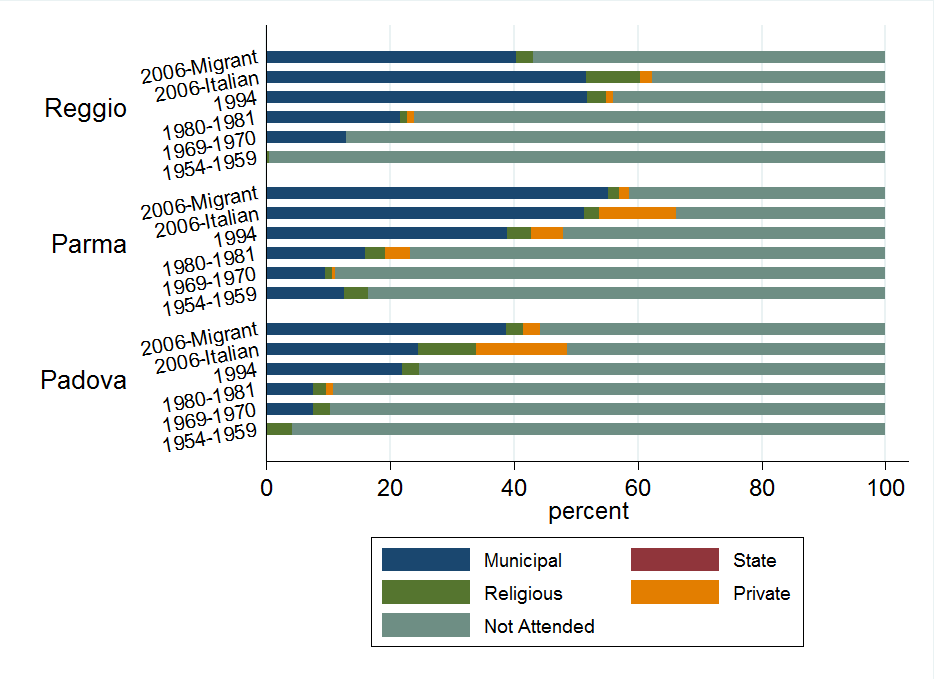
\includegraphics[width=1.15\textheight]{asiloType-Attend.png}
%\caption{{Location of the city of Parma, Reggio Emilia, and Padova, Italy.}}
\end{figure}
\end{center}
\end{frame}
%%-----------------------------------------------------------------------------------------------
\begin{frame}
\frametitle{Attendance Preschools (3-5)} 
\begin{center}
\begin{figure}
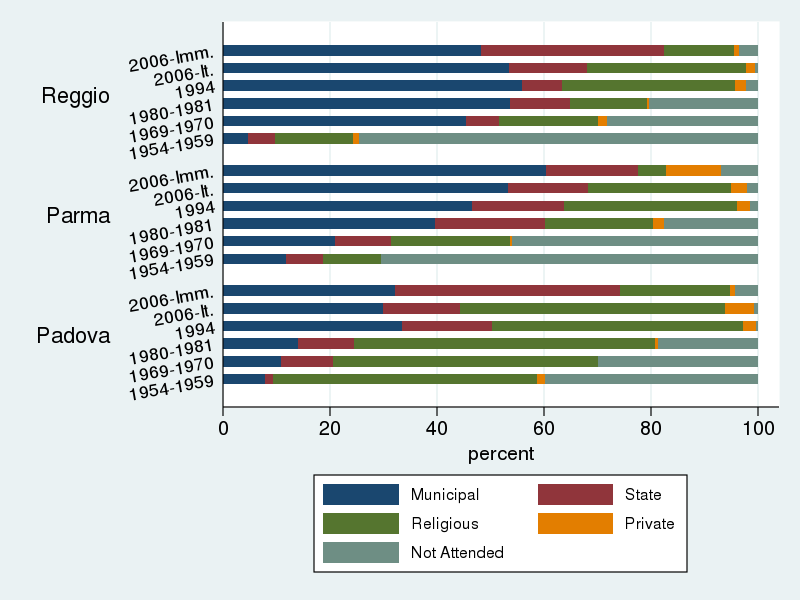
\includegraphics[width=1.15\textheight]{maternaType-Attend.png}
%\caption{{Location of the city of Parma, Reggio Emilia, and Padova, Italy.}}
\end{figure}
\end{center}
\end{frame}
%---------------------------------------------------------------------------------------------------------------------------------
\begin{frame}
% use KlmReggio\ADMINISTRATIVE DATA COLLECTION\DATI\ReggioAdminData.dta
%   tab asiloAges Cohort, column
%   tab maternaAges Cohort, column
\begin{table}[ht!]
\caption{\textbf{Number of Years Spent at Infant-Toddler Centers and Preschools, by Cohort}}
\label{tab:Years}
%\vspace{-5mm}
\begin{center}
\footnotesize
\begin{tabular}{ l c c c }
\hline\hline
& \textbf{Born 2006} & \textbf{Born 2006} & \textbf{Born 1994}\\
& \textbf{Italian} & \textbf{Immigrant} & \textbf{Italian}\\
& \textbf{(Coh. V)} & \textbf{(Coh. V)} & \textbf{(Coh. IV)}\\
\hline
&\multicolumn{3}{c}{\textit{Infant-Toddler Centers}}\\
\hline
1 Year      & 30.6\%  & 32.0\%  & 23.6\% \\[0.2em]
2 Years     & 61.7\%  & 60.3\%  & 65.1\% \\[0.2em]
3 Years     & 7.3\%   &  7.6\%  & 10.7\% \\[0.2em]
\hline
&\multicolumn{3}{c}{\textit{Preschools}}\\
\hline
1 Year      &  3.2\%  &  6.6\%  &  6.3\% \\[0.2em]
2 Years     & 28.5\%  & 30.2\%  & 28.6\% \\[0.2em]
3 Years     & 68.2\%  & 64.2\%  & 65.1\% \\[0.2em]
\hline
\end{tabular}
\end{center}
\begin{flushleft}
\tiny{{\bfseries Notes:} Source: authors' calculations from the survey data, pooled across the cities of Reggio Emilia, Parma and Padova. Years in childcare are calculated from the parental section of the children and adolescent questionnaires, subtracting age at start from age at end of attendance to infant-toddler center and preschool. Coh.=Cohort.}
\end{flushleft}
\end{table}


\end{frame}
%---------------------------------------------------------------------------------------------------------------------------------
\begin{frame}
% use KlmReggio\ADMINISTRATIVE DATA COLLECTION\DATI\ReggioAdminData.dta
%   tab asiloTime Cohort, column
%   tab maternaTime Cohort, column
\begin{table}[ht!]
\caption{\textbf{Time Spent at Infant-Toddler Centers and Preschools, by Cohort}}
\label{tab:Time}
%\vspace{-5mm}
\begin{center}
\footnotesize
\begin{tabular}{ l c c c }
\hline\hline
& \textbf{Born 2006} & \textbf{Born 2006} & \textbf{Born 1994}\\
& \textbf{Italian} & \textbf{Immigrant} & \textbf{Italian}\\
& \textbf{(Coh. V)} & \textbf{(Coh. V)} & \textbf{(Coh. IV)}\\
\hline
&\multicolumn{3}{c}{\textit{Infant-Toddler Centers}}\\
\hline
Full-Time      & 67.6\% & 85.0\% & 73.5\% \\[0.2em]
Morning only   & 29.1\% & 12.8\% & 25.1\% \\[0.2em]
Afternoon only &  0.4\% &  0.0\% &  0.0\% \\[0.2em]
Other, specify &  2.9\% &  2.3\% &  1.4\% \\
\hline
&\multicolumn{3}{c}{\textit{Preschools}}\\
\hline
Full-Time      & 86.8\% & 90.7\% & 82.8\%\\[0.2em]
Morning only   & 10.9\% &  7.1\% & 15.9\%\\[0.2em]
Afternoon only &  0.3\% &  0.4\% &  0.5\%\\[0.2em]
Other, specify &  2.0\% &  1.9\% &  0.8\%\\
\hline
\end{tabular}
\end{center}
\begin{flushleft}
\tiny{{\bfseries Notes:} Source: authors' calculations from the survey data, pooled across the cities of Reggio Emilia, Parma and Padova. The question comes from the parental section of the children and adolescent questionnaires: ``During the day, how much time did your child spend in the infant-toddler center? (tick all the answers which describe your situation)'' and ``During the day, how much time did your child spend in preschool? (tick all the answers which describe your situation)''. Coh.=Cohort.}
\end{flushleft}
\end{table}


\end{frame}
%---------------------------------------------------------------------------------------------------------------------------------
\begin{frame}
% use KlmReggio\ADMINISTRATIVE DATA COLLECTION\DATI\ReggioAdminData.dta
%   tab asiloMotive Cohort, column
\begin{table}[ht!]
\caption{\textbf{Reasons for Sending Child to Infant-Toddler Center, by Cohort}}
\label{tab:SumMotiveAsilo}
%\vspace{-5mm}
\begin{center}
 \scriptsize
 \begin{tabular}{ l c c c c }
\hline \hline
& \textbf{Born 2006} & \textbf{Born 2006} & \textbf{Born 1994} & \textbf{Total} \\
& \textbf{Italian} & \textbf{Immigrant} & \textbf{Italian} & \textbf{} \\
% & \textbf{(Coh. V)} % & \textbf{(Coh. V)} & \textbf{(Coh. IV)} & \textbf{} \\
\hline
Parents were busy working           & 79.9\% & 65.4\% & 85.4\% & 80.0\% \\[0.2em]
To socialize with other children    & 52.9\% & 42.9\% & 47.7\% & 49.7\% \\[0.2em]
Important for her development       & 50.8\% & 51.9\% & 47.4\% & 49.7\% \\[0.2em]
No close-by grandparents            & 17.8\% & 30.8\% & 15.7\% & 18.8\% \\[0.2em]
Younger siblings required attention &  3.1\% &  6.0\% &  3.0\% &  3.4\% \\[0.2em]
Don't remember                      &  0.0\% &  1.5\% &  0.6\% &  0.4\% \\[0.2em]
Other, specify                      &  2.3\% &  7.5\% &  0.3\% &  2.3\% \\[0.2em]
No response                         &  0.4\% &  0.8\% &  0.3\% &  0.4\% \\
\hline
Observations                        &   522 &   133 &   363 & 1,018 \\
\hline
\end{tabular}
\end{center} \begin{flushleft}
\tiny{{\bfseries Notes:} Source: authors' calculations from the survey data, pooled across the cities of Reggio Emilia, Parma and Padova. The question comes from the parental section of the children and adolescent questionnaires: ``For what reasons did your child attend the infant-toddler center? (tick all answers which describe your situation)''. Cells display the percentage of caregivers who report the stated reason. Coh.=Cohort.}
\end{flushleft} \end{table}

\end{frame}
%---------------------------------------------------------------------------------------------------------------------------------
\begin{frame}
\begin{table}[ht!]
\caption{\textbf{Reasons for Not Sending Child to Infant-Toddler Center, by Cohort}}
\label{tab:SumMotiveNOAsilo}
%\vspace{-5mm}
\begin{center}
 \scriptsize
 \begin{tabular}{ l c c c c }
\hline\hline
& \textbf{Born 2006} & \textbf{Born 2006} & \textbf{Born 1994} & \textbf{Total} \\
& \textbf{Italian} & \textbf{Immigrant} & \textbf{Italian} & \textbf{} \\
% & \textbf{(Coh. V)} % & \textbf{(Coh. V)} & \textbf{(Coh. IV)} & \textbf{} \\
\hline
Home best for her development    & 37.7\% & 38.5\% & 37.4\% & 37.7\% \\[0.2em]
Grandparents were available      & 27.9\% & 06.1\% & 28.1\% & 24.7\% \\[0.2em]
Child too young                  & 24.6\% & 26.3\% & 16.5\% & 20.9\% \\[0.2em]
Too expensive                    & 16.8\% & 53.4\% & 08.0\% & 18.1\% \\[0.2em]
Child did not want to go         &  2.0\% &  0.7\% &  0.0\% &  0.8\% \\[0.2em]
Desired placement not achieved   &  3.6\% &  4.7\% &  4.4\% &  4.2\% \\[0.2em]
Close-by centers of low quality  &  0.3\% &  0.0\% &  0.2\% &  0.2\% \\[0.2em]
Don't remember                   &  2.5\% &  2.0\% &  3.6\% &  3.0\% \\[0.2em]
Other, specify                   & 15.9\% & 16.9\% & 13.9\% & 15.1\% \\[0.2em]
No response                      &  2.0\% &  1.3\% &  4.9\% &  3.3\% \\
\hline
Observations                     &  358  &  148  &  473  &  979\\
\hline
\end{tabular}
\end{center} \begin{flushleft}
\tiny{{\bfseries Notes:} Source: authors' calculations from the survey data, pooled across the cities of Reggio Emilia, Parma and Padova. The question comes from the parental section of the children and adolescent questionnaires: ``For what reasons your child did not attend the infant-toddler center? (tick all answers which describe your situation)''. Cells display the percentage of caregivers who report the stated reason. Coh.=Cohort.}
\end{flushleft} \end{table}

\end{frame}
%---------------------------------------------------------------------------------------------------------------------------------
\begin{frame}
% use KlmReggio\ADMINISTRATIVE DATA COLLECTION\DATI\ReggioAdminData.dta
%   tab maternaMotive Cohort, column
\begin{table}[ht!]
\caption{\textbf{Reasons for Sending Child to Preschool, by Cohort}}
\label{tab:SumMotiveMaterna}
%\vspace{-5mm}
\begin{center}
 \scriptsize
 \begin{tabular}{ l c c c c }
\hline\hline
& \textbf{Born 2006} & \textbf{Born 2006} & \textbf{Born 1994} & \textbf{Total} \\
& \textbf{Italian} & \textbf{Immigrant} & \textbf{Italian} & \textbf{} \\
% & \textbf{(Coh. V)} % & \textbf{(Coh. V)} & \textbf{(Coh. IV)} & \textbf{} \\
\hline
Important for her development       & 68.5\% & 69.8\% & 62.9\% & 66.4\% \\[0.2em]
Parents were busy working           & 62.2\% & 48.9\% & 59.3\% & 59.2\% \\[0.2em]
To socialize with other children    & 61.5\% & 58.6\% & 57.7\% & 59.5\% \\[0.2em]
No close-by grandparents            & 12.3\% & 31.0\% & 09.2\% & 13.6\% \\[0.2em]
Younger siblings required attention &  6.0\% & 16.0\% &  4.1\% &  6.6\% \\[0.2em]
Don't remember                      &  1.3\% &  0.4\% &  0.7\% &  0.9\% \\[0.2em]
Other, specify                      &  0.9\% & 10.4\% &  1.2\% &  2.3\% \\[0.2em]
No response                         &  0.6\% &  0.4\% &  0.9\% &  0.7\% \\
\hline
Observations                        &   868 &   268 &   488 & 1,959 \\
\hline
\end{tabular}
\end{center} \begin{flushleft}
\tiny{{\bfseries Notes:} Source: authors' calculations from the survey data, pooled across the cities of Reggio Emilia, Parma and Padova. The question comes from the parental section of the children and adolescent questionnaires: ``For what reasons did your child attend the preschool? (tick all answers which describe your situation)''. Cells display the proportion of caregivers who report the stated reason. Coh.=Cohort.}
\end{flushleft} \end{table}


\end{frame}
%%---------------------------------------------------------------------------------------------------------------------------------
%\begin{frame}
%\input{SumMotiveNOMaterna}
%\end{frame}
%---------------------------------------------------------------------------------------------------------------------------------
\begin{frame}
\begin{table}[ht!]
\footnotesize
\caption{\textbf{Important Aspects of Infant-Toddler Center, by Cohort}}
\label{tab:SumImportantAsilo}
%\vspace{-5mm}
\begin{center}
 \tiny 
 \begin{tabular}{ l c c c c c c c }
\hline\hline
& \textbf{Born} & \textbf{Born} & \textbf{Born} & \textbf{Born} & \textbf{Born} & \textbf{Born} & \textbf{Total} \\
& \textbf{2006-It.} & \textbf{2006-Imm.} & \textbf{1994} & \textbf{1980-81} & \textbf{1969-70} & \textbf{1954-59} & \textbf{} \\
% & \textbf{(Coh. V)} % & \textbf{(Coh. V)} & \textbf{(Coh. IV)} & \textbf{(Coh. III)} & \textbf{(Coh. II)} & \textbf{(Coh. I)} \textbf{} \\
\hline
Play with other children     & 86.2\% & 75.9\% & 84.0\% & 69.2\% & 51.1\% & 18.2\% & 78.8\%\\[0.2em]
Teachers taught autonomy     & 64.6\% & 46.6\% & 62.0\% & 34.6\% & 24.5\% & 40.9\% & 55.0\%\\[0.2em]
Nice setting with playground & 55.6\% & 45.9\% & 52.9\% & 55.1\% & 42.5\% & 63.6\% & 52.9\%\\[0.2em]
No good memories             &  1.3\% &  0.0\% &  2.5\% &  3.8\% &  6.4\% &  0.0\% &  2.2\%\\[0.2em]
No memories                  &  0.2\% &  6.8\% &  1.9\% &  9.6\% & 14.9\% &  9.1\% &  3.7\%\\[0.2em]
Other, specify               &  3.4\% &  3.8\% &  1.4\% &  1.9\% &  0.0\% &  4.5\% &  2.5\%\\[0.2em]
No response                  &  0.2\% &  0.8\% &  0.3\% &  0.0\% &  0.0\% &  0.0\% &  0.2\%\\
\hline
Observations                 &   522 &   133 &   363 &   156 &    94 &    22 & 1,290 \\
\hline
\end{tabular}
\end{center} \begin{flushleft}
\tiny{{\bfseries Notes:} Source: authors' calculations from the survey data, pooled across the cities of Reggio Emilia, Parma and Padova. The question comes from the parental section of the children and adolescent questionnaires: ``Which aspects of the experience at the infant-toddler center do you think have been more important for your child? (tick all answers which describe your situation)''; and from the adults questionnaires: ``Which aspects of the experience at the infant-toddler center do you remember as more important? (tick all answers which describe your situation)''. Cells display the proportion of caregivers or adults who report the stated aspect. Coh.=Cohort. It.=Italian. Imm.=Immigrant.}
\end{flushleft} \end{table}

\end{frame}
%---------------------------------------------------------------------------------------------------------------------------------
\begin{frame}
% use KlmReggio\ADMINISTRATIVE DATA COLLECTION\DATI\ReggioAdminData.dta
\begin{table}[ht!]
\footnotesize
\caption{\textbf{Important Aspects of Preschool, by Cohort}}
\label{tab:SumImportantMaterna}
%\vspace{-5mm}
\begin{center}
 \tiny 
 \begin{tabular}{ l c c c c c c c }
\hline \hline
& \textbf{Born} & \textbf{Born} & \textbf{Born} & \textbf{Born} & \textbf{Born} & \textbf{Born} & \textbf{Total} \\
& \textbf{2006-It.} & \textbf{2006-Imm.} & \textbf{1994} & \textbf{1980-81} & \textbf{1969-70} & \textbf{1954-59} & \textbf{} \\
% & \textbf{(Coh. V)} % & \textbf{(Coh. V)} & \textbf{(Coh. IV)} & \textbf{(Coh. III)} & \textbf{(Coh. II)} & \textbf{(Coh. I)} \textbf{} \\
\hline
Play with other children     & 84.6\% & 77.6\% & 84.7\% & 69.8\% & 61.1\% & 56.7\% & 76.0\%\\[0.2em]
Teachers taught autonomy     & 74.3\% & 62.7\% & 67.6\% & 33.2\% & 36.0\% & 22.7\% & 54.7\%\\[0.2em]
Nice setting with playground & 51.8\% & 56.0\% & 47.6\% & 58.0\% & 54.6\% & 45.3\% & 52.4\%\\[0.2em]
No good memories             &  2.0\% &  0.0\% &  1.1\% &  3.2\% &  5.8\% &  8.1\% &  2.7\%\\[0.2em]
No memories                  &  0.2\% &  0.7\% &  0.6\% &  4.1\% &  5.4\% & 10.5\% &  2.5\%\\[0.2em]
Other, specify               &  3.6\% &  6.3\% &  2.3\% &  1.9\% &  1.3\% &  4.1\% &  2.8\%\\[0.2em]
No response                  &  0.6\% &  0.7\% &  0.5\% &  0.2\% &  0.2\% &  0.0\% &  0.4\%\\
\hline
Observations                 &   868 &   268 &   823 &   633 &   520 &   172 &  3,284  \\
\hline
\end{tabular}
\end{center} \begin{flushleft}
\tiny{{\bfseries Notes:} Source: authors' calculations from the survey data, pooled across the cities of Reggio Emilia, Parma and Padova. The question comes from the parental section of the children and adolescent questionnaires: ``Which aspects of the experience at the preschool do you think have been more important for your child? (tick all answers which describe your situation)''; and from the adults questionnaires: ``Which aspects of the experience at the preschool do you remember as more important? (tick all answers which describe your situation)''. Cells display the proportion of caregivers or adults who report the stated aspect. Coh.=Cohort. It.=Italian. Imm.=Immigrant.}
\end{flushleft} \end{table}


\end{frame}

%: Appendix %-----------------------------------------------------------------------------------------------
\appendix
%-----------------------------------------------------------------------------------------------
\begin{frame}
\begin{center}
\begin{figure}
\includegraphics[width=0.9\textheight]{Bimbo}
\end{figure}

\vspace{1ex}

{\Huge{Thanks!}}
\end{center}
\end{frame} 
%% -----------------------------------------------------------------------------------------------


%: Infant-toddler centers %----------------------------------------------------------------
%%-----------------------------------------------------------------------------------------------
\begin{frame}
\frametitle{Infant-Toddler Centers (0-3) in Italy}
\begin{center}
\begin{figure}
\includegraphics[width=1.0\textheight]{Childcare.pdf} \label{fig:AttendaceAsiloIT}
\caption{No. of children enrolled/no. of children 0-3 [2009].}
\end{figure}
\end{center}
\hyperlink{frame:ECE_IT}{\beamergotobutton{back}}
\end{frame} 
%%-----------------------------------------------------------------------------------------------
\begin{frame}
\frametitle{Public and Private Infant-toddler Centers (0-3) in Italy}
\begin{center}
\begin{figure}
\includegraphics[width=1.0\textheight]{PublPriv.pdf}  \label{fig:PrivateAsiloIT}
\caption{No. of child care centers for children 0-3 [2010].}
\end{figure}
\end{center}
\hyperlink{frame:ECE_IT}{\beamergotobutton{back}}
\end{frame} 

%: Maps %----------------------------------------------------------------
%%-----------------------------------------------------------------------------------------------
\begin{frame}
\frametitle{Reggio Children Approach Around the World}
\hyperlink{frame:philosphy}{\beamergotobutton{back}}
\begin{center}
\begin{figure}
%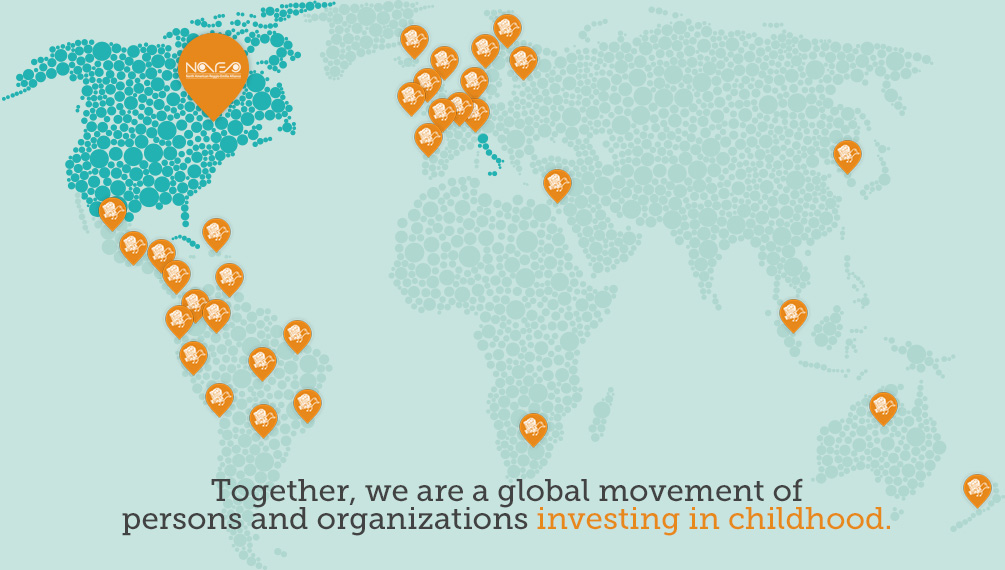
\includegraphics[height=0.7\textheight]{ReggioWorldMap.jpg}
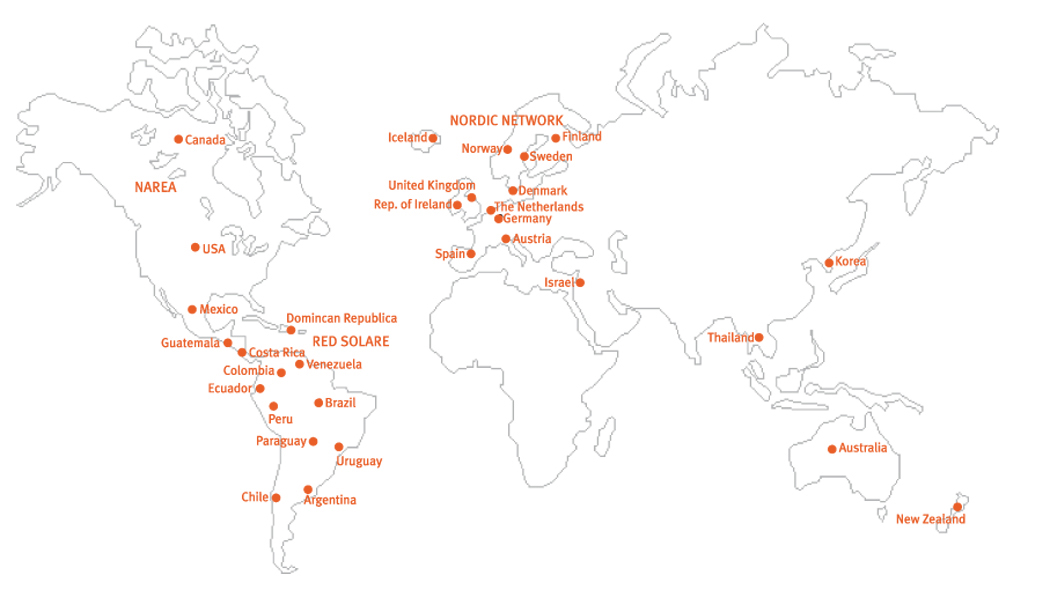
\includegraphics[height=0.7\textheight]{network3.jpg}
\label{fig:World} 
\caption{{Location of Reggio inspired schools and associations}}
\end{figure}
\end{center}
\end{frame} 
%%-----------------------------------------------------------------------------------------------
\begin{frame}
\frametitle{ITC and Preschools in Reggio Emilia}
\begin{center}
\begin{figure}
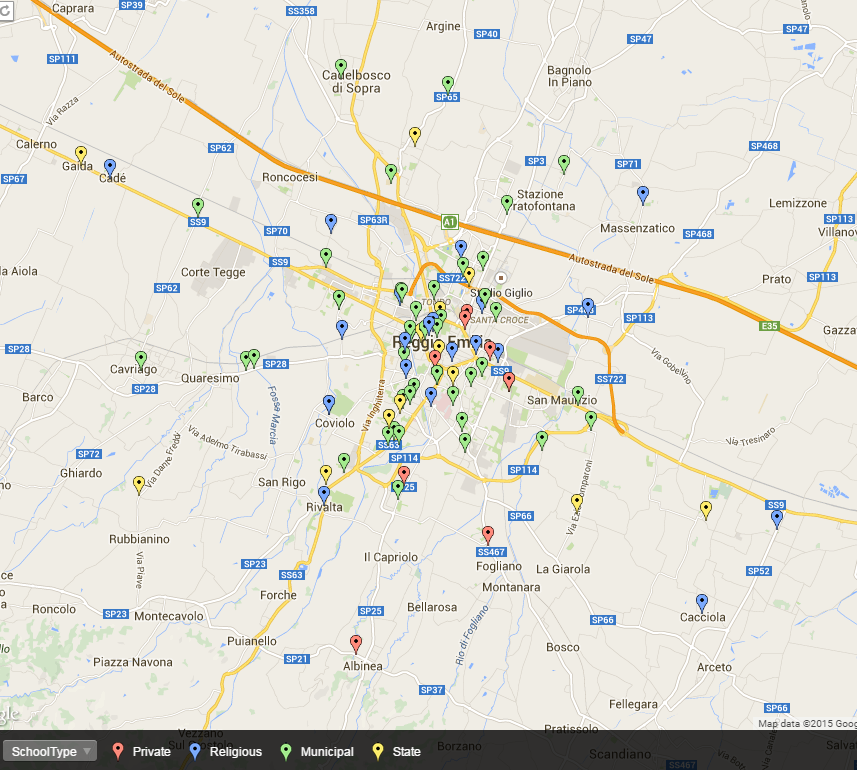
\includegraphics[height=0.9\textheight]{ReggioSchools.png}
\label{fig:ReggioSchools} 
\hyperlink{frame:treatment}{\beamergotobutton{back}}
%\caption{{Location of Reggio inspired schools and associations}}
\end{figure}
\end{center}
\end{frame} 
%%-----------------------------------------------------------------------------------------------
\begin{frame}
\frametitle{ITC and Preschools in Parma}
\begin{center}
\begin{figure}
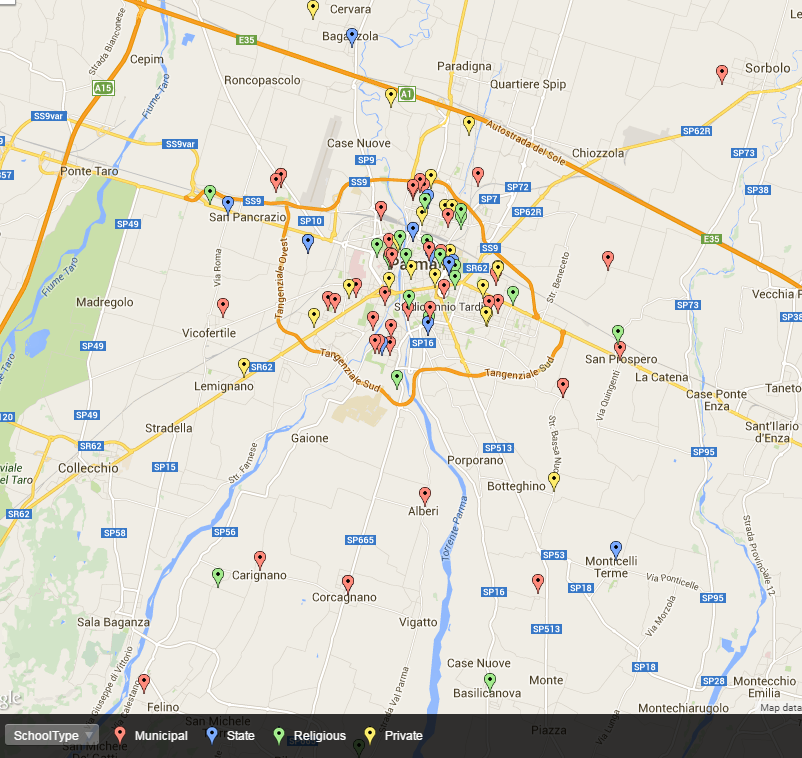
\includegraphics[height=0.9\textheight]{ParmaSchools.png}
\label{fig:ParmaSchools} 
\hyperlink{frame:treatment}{\beamergotobutton{back}}
%\caption{{Location of Reggio inspired schools and associations}}
\end{figure}
\end{center}
\end{frame} 
%%-----------------------------------------------------------------------------------------------
\begin{frame}
\frametitle{ITC and Preschools in Padova}
\begin{center}
\begin{figure}
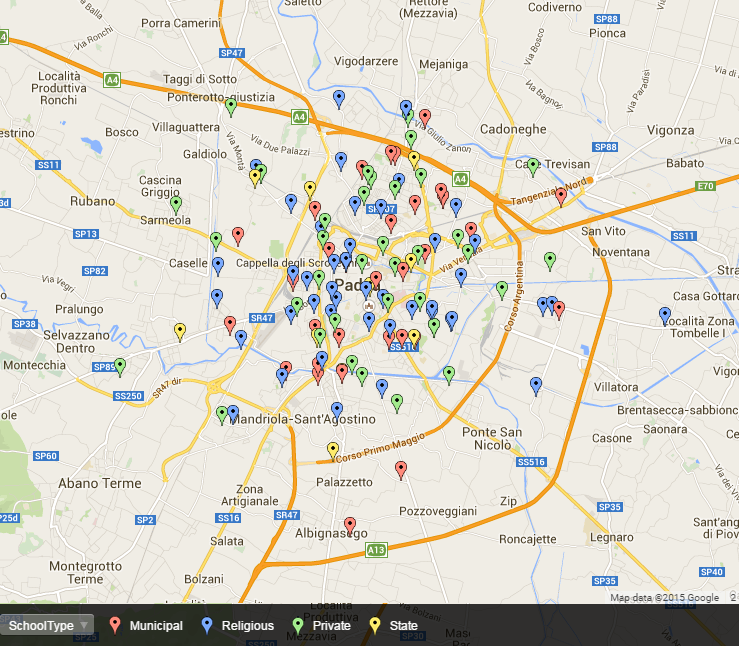
\includegraphics[height=0.9\textheight]{PadovaSchools.png}
\label{fig:PadovaSchools} 
\hyperlink{frame:treatment}{\beamergotobutton{back}}
%\caption{{Location of Reggio inspired schools and associations}}
\end{figure}
\end{center}
\end{frame} 

%: Reference %-----------------------------------------------------------------------------------------------%
\begin{frame}[allowframebreaks]  %<beamer:0> hides the frames (but gives error messages; [allowframebreaks] adjusts the number of slides
\frametitle{References}
\begin{tiny}
\bibliographystyle{apalike}
\bibliography{/home/UZH/pbirol/Documents/papers/library}  %from laptop
\end{tiny}
\end{frame}
%%-%-%-%-%-%-%-%-%-%-%-%-%-%-%
\end{document}
